\documentclass[12pt]{article}
\usepackage[margin=2.5cm]{geometry}
\usepackage{enumerate}
\usepackage{amsfonts}
\usepackage{amsmath}
\usepackage{fancyhdr}
\usepackage{amsmath}
\usepackage{amssymb}
\usepackage{amsthm}
\usepackage{mdframed}
\usepackage{graphicx}
\usepackage{subcaption}
\usepackage{adjustbox}
\usepackage{listings}
\usepackage{xcolor}
\usepackage{booktabs}
\usepackage[utf]{kotex}
\usepackage{hyperref}

\definecolor{codegreen}{rgb}{0,0.6,0}
\definecolor{codegray}{rgb}{0.5,0.5,0.5}
\definecolor{codepurple}{rgb}{0.58,0,0.82}
\definecolor{backcolour}{rgb}{0.95,0.95,0.92}

\lstdefinestyle{mystyle}{
    backgroundcolor=\color{backcolour},
    commentstyle=\color{codegreen},
    keywordstyle=\color{magenta},
    numberstyle=\tiny\color{codegray},
    stringstyle=\color{codepurple},
    basicstyle=\ttfamily\footnotesize,
    breakatwhitespace=false,
    breaklines=true,
    captionpos=b,
    keepspaces=true,
    numbers=left,
    numbersep=5pt,
    showspaces=false,
    showstringspaces=false,
    showtabs=false,
    tabsize=1
}

\lstset{style=mystyle}

\pagestyle{fancy}
\renewcommand{\headrulewidth}{0.4pt}
\lhead{Team Treehouse}
\rhead{Querying Relational Databases Part 1 Notes}

\begin{document}
\title{Querying Relational Databases Part 1 Notes}
\author{Team Treehouse}
\maketitle

\bigskip

\section{Why We Make Databases "Relational"}

\bigskip

\begin{itemize}
    \item Organizes data into related tables by their context and meaning
    \item Has benefits
    \begin{itemize}
        \item Maximizes Storage
        \item Better application functionality
        \item Clenear, richer data for business reporting
    \end{itemize}
\end{itemize}

\bigskip

\section{Database Normalization}

\bigskip

\begin{itemize}
    \item \textbf{Normalization:} Is the process of eliminating redundant or
    repeating data in a database
\end{itemize}

\bigskip

\section{How Normalization Helps Us}

\bigskip

\begin{itemize}
    \item Drastically reduces the amount of spaces required
    \begin{itemize}
        \item Old days (And today too!!) $\to$ is crucial
    \end{itemize}

    \begin{center}
    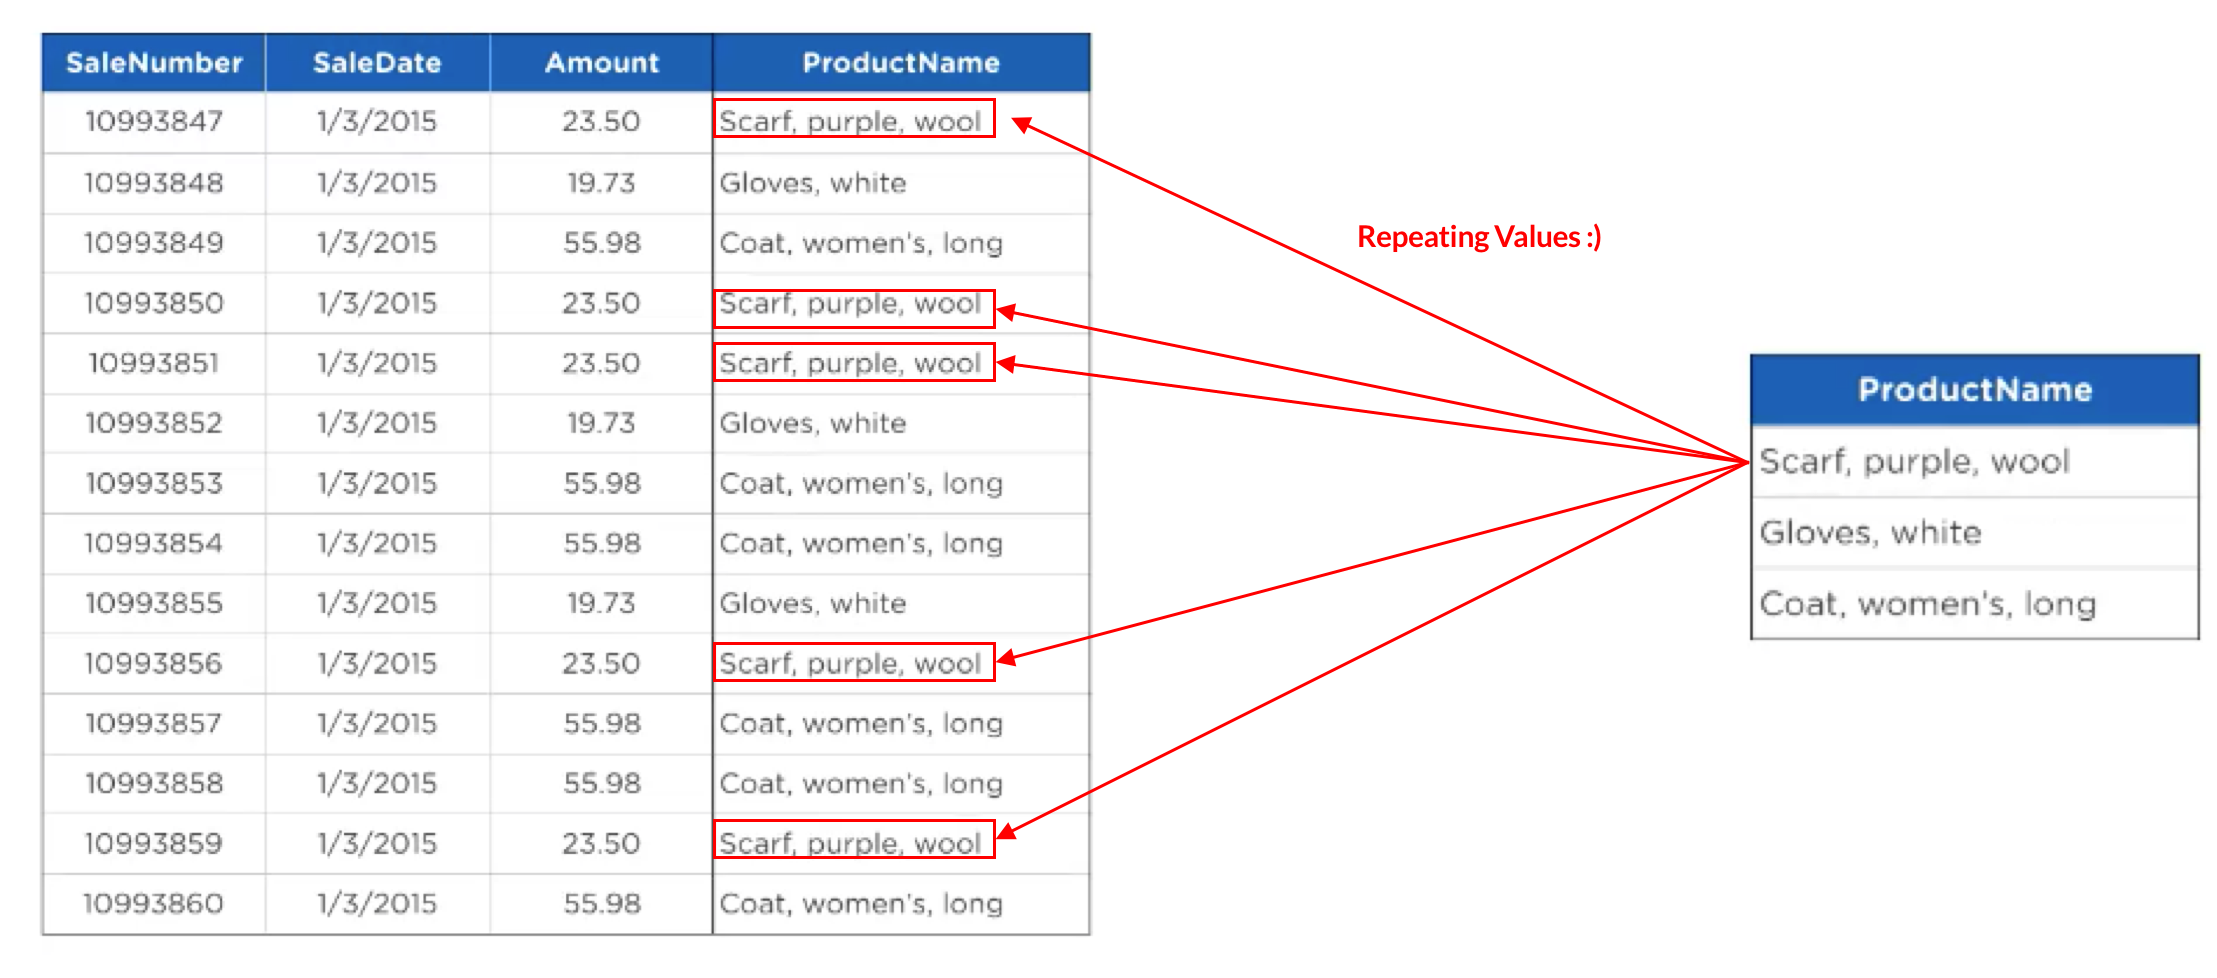
\includegraphics[width=0.8\linewidth]{images/part_1_notes_1.png}
    \end{center}
    \item Reduces update time
    \begin{itemize}
        \item Update affects millions
    \end{itemize}
\end{itemize}

\bigskip

\section{Quiz 1}

\bigskip

\begin{enumerate}[1.]
    \item

    Which of these is NOT a benefit of a relational database?

    \bigskip

    \begin{enumerate}[A.]
        \item Saves disk space as much as possible.
        \item Data conveniently stored in one table.
        \item Eliminates data modification anomalies and increases data integrity.
    \end{enumerate}

    \bigskip

    \textbf{Answer:} B

    \item

    What is Normalization?

    \bigskip

    \begin{enumerate}[A.]
        \item The process of writing queries against a relational database.
        \item The process of designing a relational database.
        \item The process of combining many tables into one.
    \end{enumerate}

    \bigskip

    \textbf{Answer:} B

    \item

    Which CRUD operation benefits most from a well normalized database design?

    \bigskip

    \begin{enumerate}[A.]
        \item INSERT
        \item UPDATE
        \item DELETE
        \item All of These
    \end{enumerate}

    \bigskip

    \textbf{Answer:} D

    \item

    When were relational databases first conceptualized?

    \bigskip

    \begin{enumerate}[A.]
        \item The 1990s
        \item The 1970s
        \item The 1950s
    \end{enumerate}

    \bigskip

    \textbf{Answer:} B

    \item

    Where does the term “relational databases” come from?

    \bigskip

    \begin{enumerate}[A.]
        \item A relational database is the best way for a computer system to “relate” to the outside world.
        \item There is an implied inheritance between parent and child databases, thus the phrase “relational”
        \item Tables in a relational database are linked -- or “related” -- via fields that they have in common.
    \end{enumerate}

    \bigskip

    \textbf{Answer:} C

\end{enumerate}

\bigskip

\section{Set Theory and Relational Databases}

\bigskip

\begin{itemize}
    \item Intersection
    \begin{itemize}
        \item Is a set of items in common
    \end{itemize}

    \begin{center}
    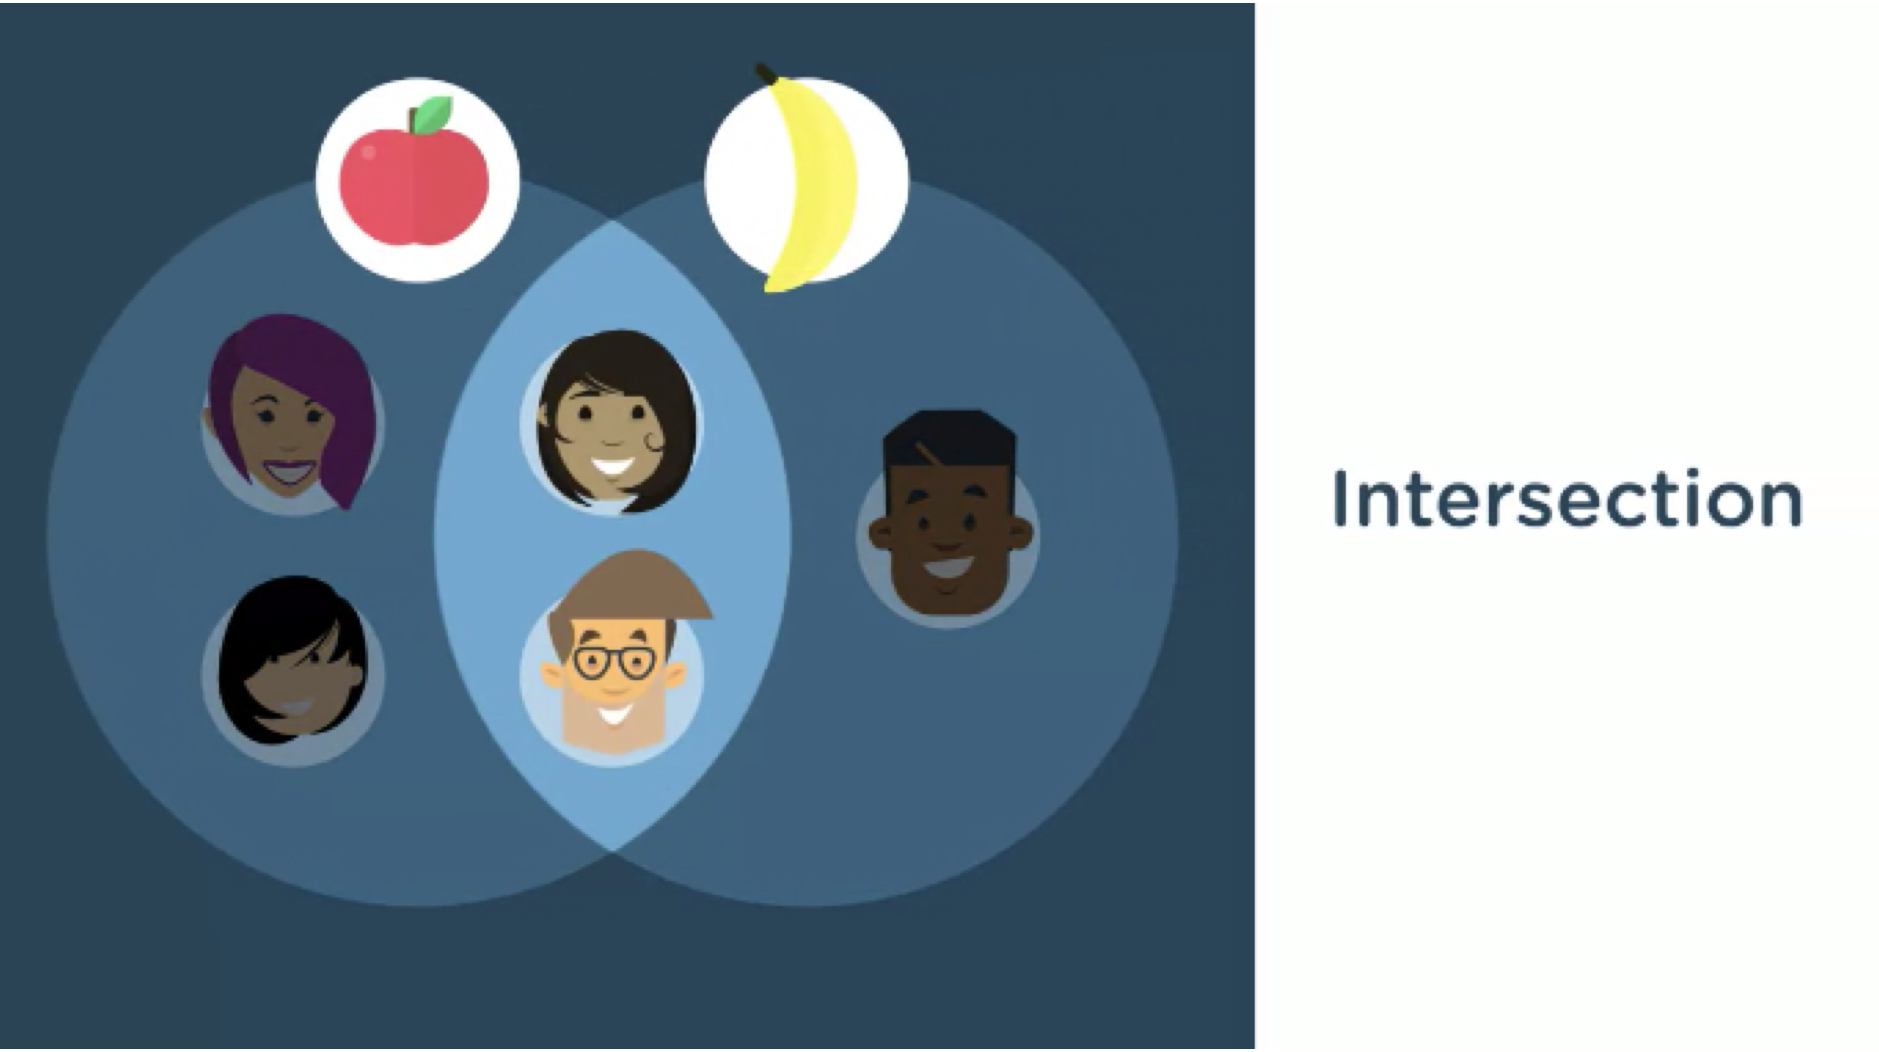
\includegraphics[width=0.8\linewidth]{images/part_1_notes_2.png}
    \end{center}

    \item Union
    \begin{itemize}
        \item Is all non-repeating values in two sets
    \end{itemize}

    \begin{center}
    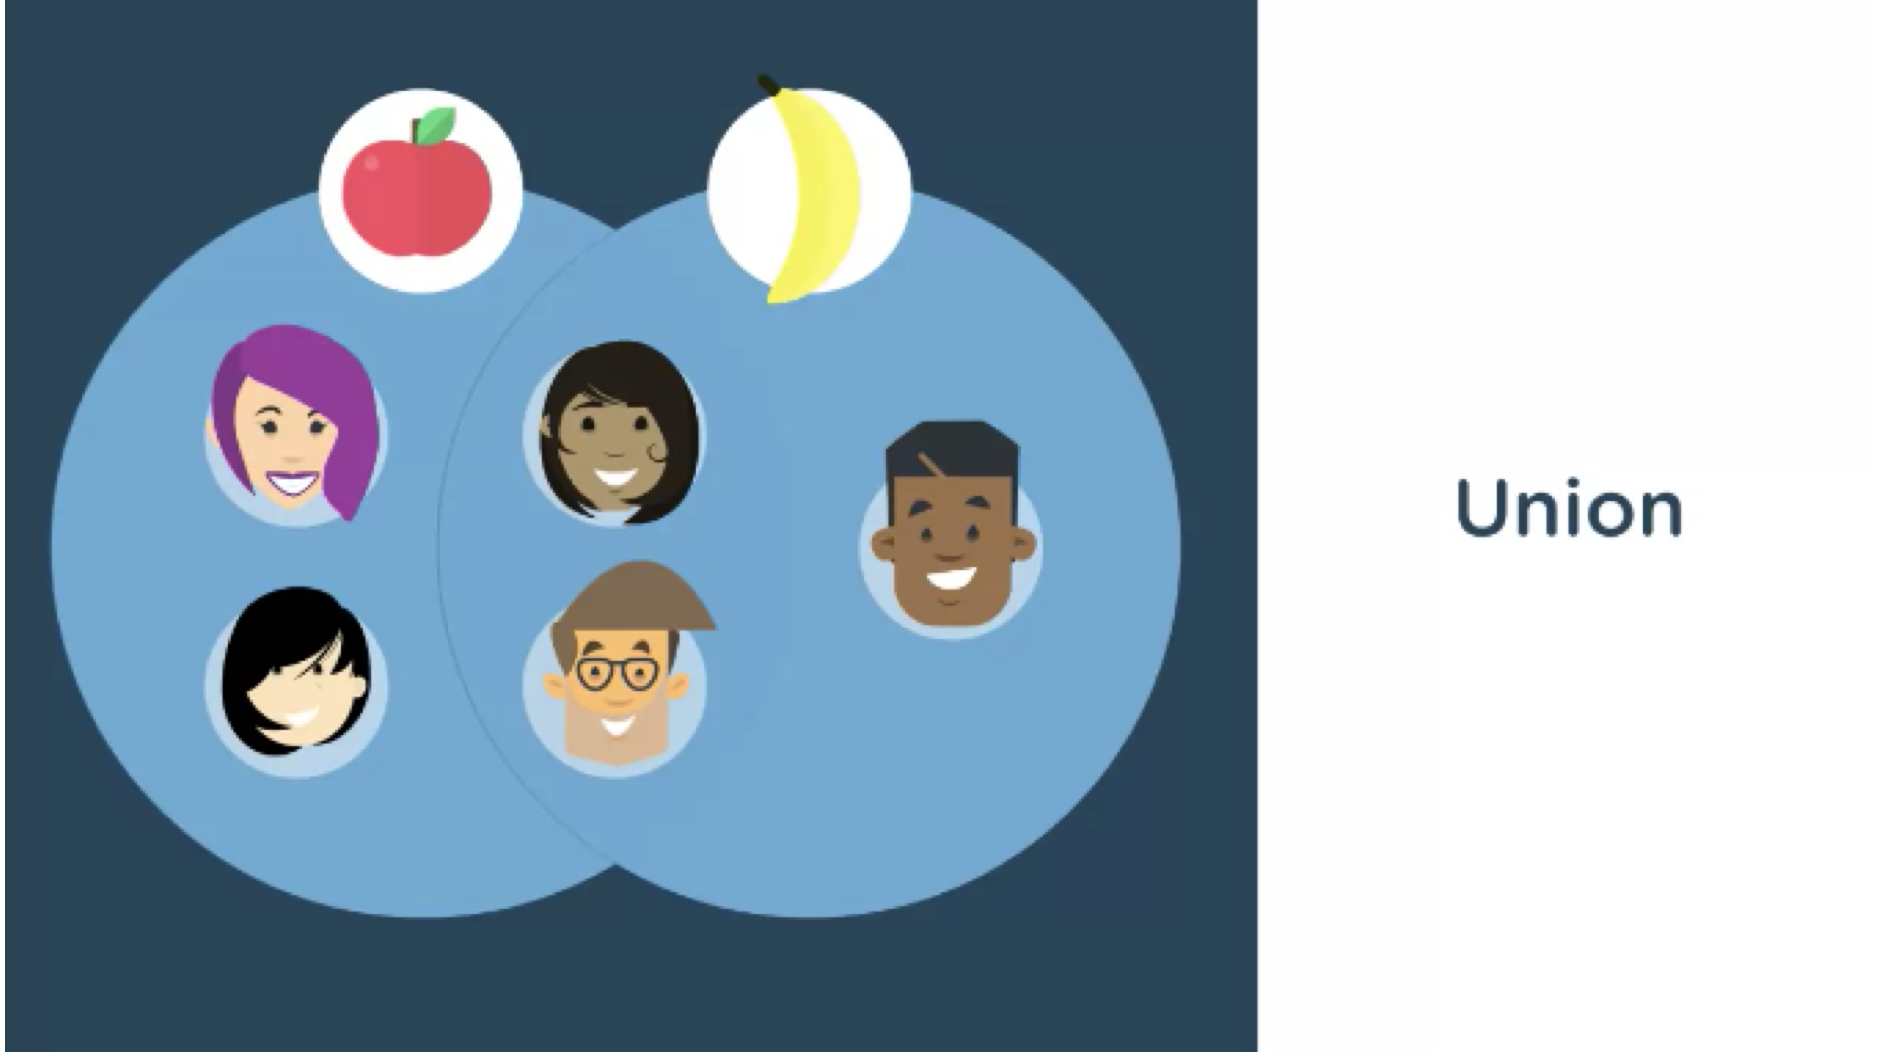
\includegraphics[width=0.8\linewidth]{images/part_1_notes_3.png}
    \end{center}

    \item Except
    \begin{itemize}
        \item Is a set of elements that are not in common

    \begin{center}
    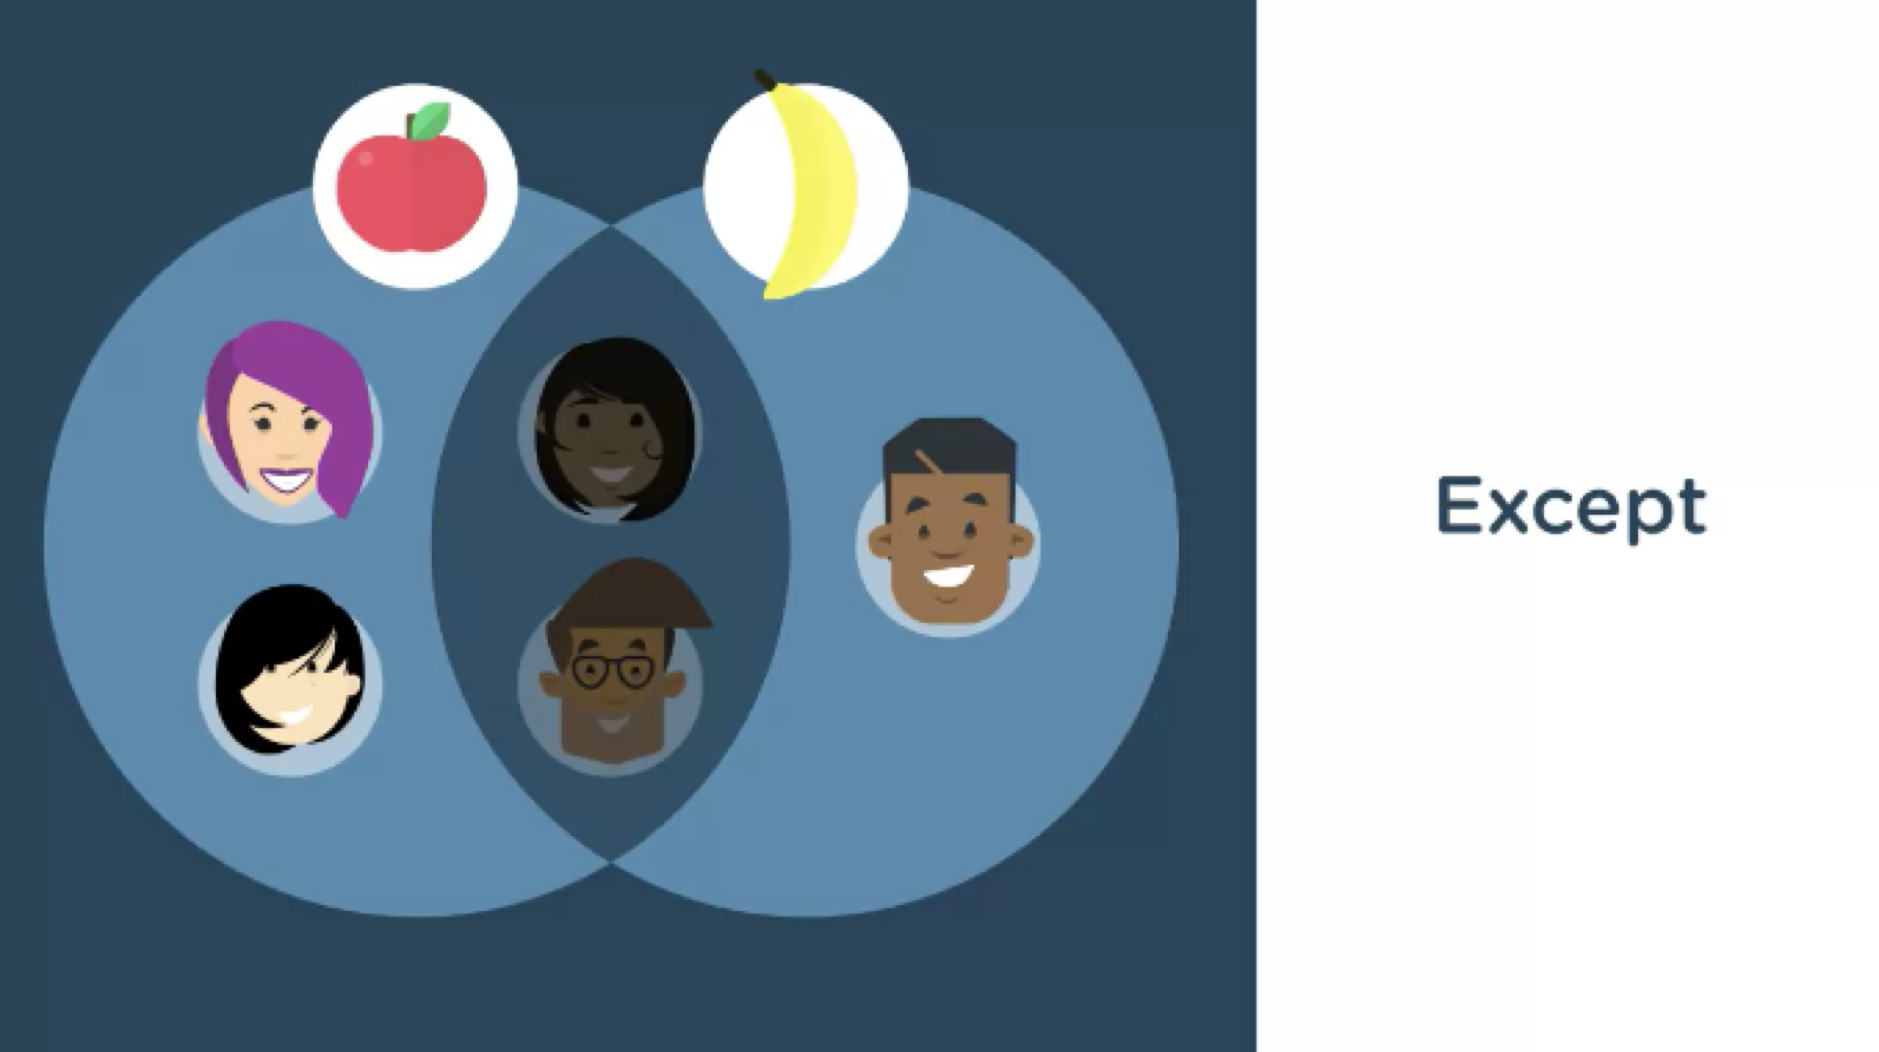
\includegraphics[width=0.8\linewidth]{images/part_1_notes_4.png}
    \end{center}

    \end{itemize}
\end{itemize}

\end{document}